%
% TODO 
%  - colocar legendas nas figuras, melhorar as figuras
%  - verificar a palavra "agente"
% 


\documentclass[a4paper, twocolumn, 12pt]{article}
\pagestyle{empty}

\usepackage[portuguese]{babel}
\usepackage[T1]{fontenc}
\usepackage[utf8]{inputenc}

\usepackage{booktabs}

%\usepackage{natbib}
%\usepackage{pstricks}
%\usepackage{pst-plot}
\usepackage[pdftex]{graphicx}
\usepackage{url}
%\usepackage[top=1cm,bottom=1cm,left=1cm,right=1cm]{geometry}
%\usepackage{multicol}

%\usepackage{amssymb,amsmath}
%\usepackage{extraipa}
%\usepackage{euler}
\everymath{\displaystyle}

\author{André Wagner}
\title{Utilização de Algoritmo de Busca Cega em Cálculo de Relacionamentos Sociais}

\begin{document}

\maketitle

%%%%%%%%%%%%%%%%%%%%%%%%%%%%%%%%%%%%%%%%%%%%%%%%%%%%%%%%%%%%%%%%%%%%%%%%%%

\section{Introdução}

Alguns artigos \cite{park,lazarsfeld1954fsp} mostram que informações a respeito de uma pessoa podem ser inferidas através de informações de seus amigos, uma vez que existe um tendência que uma pessoa tenha ao menos algumas preferências semelhantes a seus amigos.

No entanto, também é interessante que seja levado em conta a influência dos amigos dos amigos, uma vez que as preferências destes também terão alguma semelhança com as da pessoa original,  e podem ser fonte de informações valiosas para o cálculo de inferências.

Este artigo busca calcular o grau de influência que há entre duas pessoas, mesmo que elas não conheçam uma à outra, mas tenham um terceiro em comum. O algoritmo utilizado para este fim é o algoritmo de busca cega.

%%%%%%%%%%%%%%%%%%%%%%%%%%%%%%%%%%%%%%%%%%%%%%%%%%%%%%%%%%%%%%%%%%%%%%%%%%

\section{Desenvolvimento}

Foi desenvolvido um programa que realiza este cálculo através de uma base de dados de \emph{eventos de relacionamento}, onde cada evento é composto dos nomes das duas pessoa e de um valor para este evento, que deve estar entre 0 e 1. O valor define a importância do evento. Por exemplo, uma simples troca de e-mails entre duas pessoas define um evento de pouca importância (ou seja, não significa muito para definir que estas pessoas tenham um relacionamento forte), mas o fato de duas pessoas realizarem um trabalho em conjunto tem um valor maior.

O programa soma os valores dos eventos que ocorreram entre cada par de pessoas (o \emph{grau de relacionamento} entre elas), e monta um grafo contendo a \emph{rede de relacionamentos}, onde os pesos dos vértices equivalem ao grau de relacionamento.

Levando em consideração a base de dados de eventos abaixo, um exemplo de grafo seria o representado na Figura~\ref{fig:exemplo1}.

\begin{verbatim}
Andre Morgana 0.15
Tiago Andre 0.61
Lucas Tiago 0.74
Andre Tiago 0.84
Morgana Tiago 0.58
\end{verbatim}

\begin{figure}
  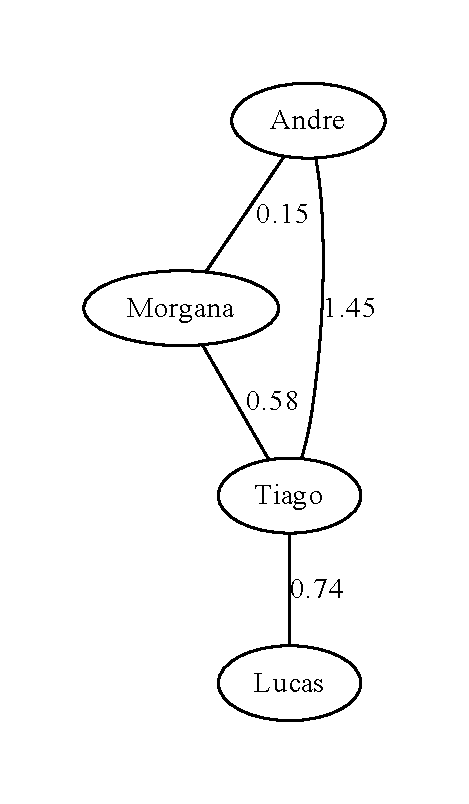
\includegraphics[width=0.5\textwidth]{teste.pdf}
  \caption{Exemplo de rede de relacionamentos}
  \label{fig:exemplo1}
\end{figure}

Outros exemplos mais complexos podem ser criados, uma vez que o número de usuários é livre, como na Figura~\ref{fig:exemplo2}.

\begin{figure}
  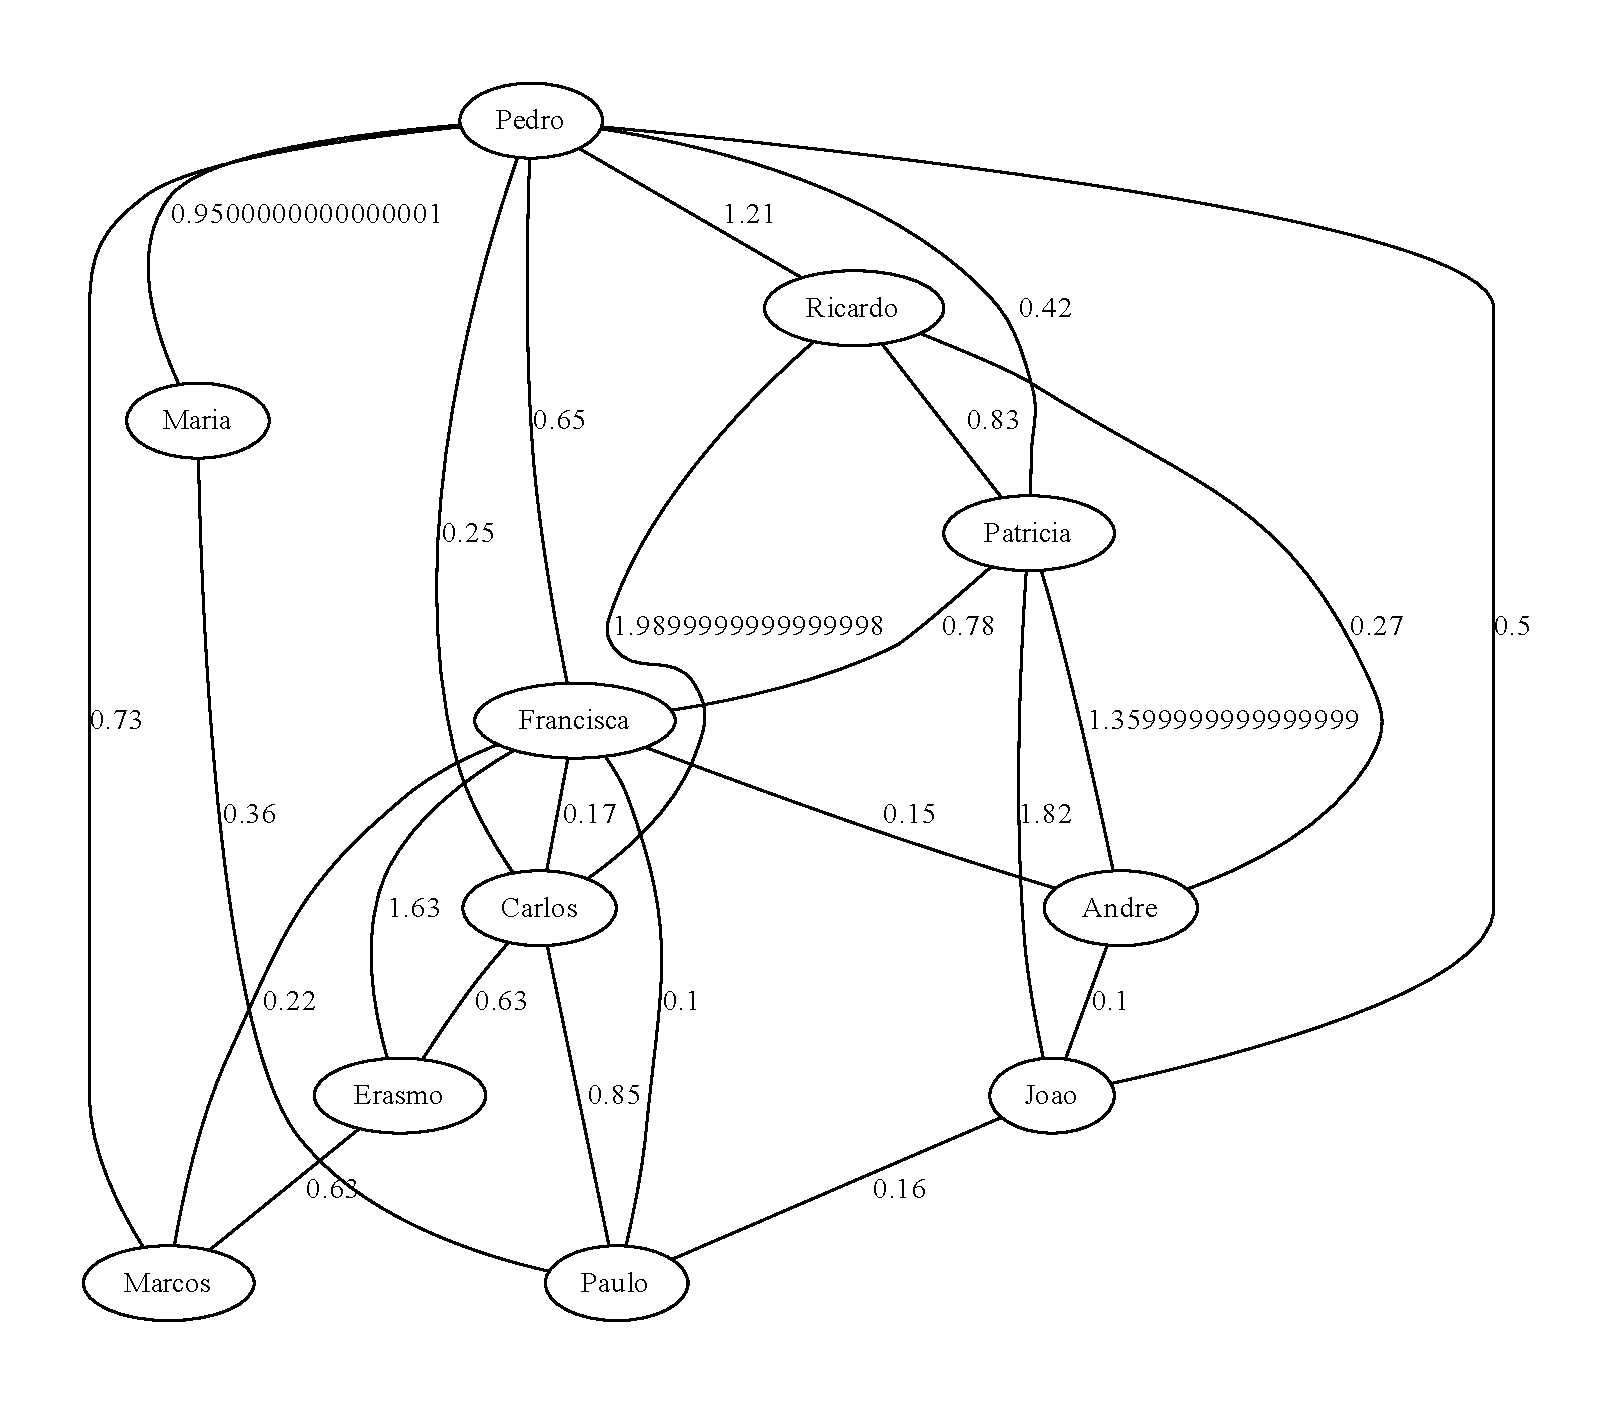
\includegraphics[width=0.5\textwidth]{teste2.pdf}
  \caption{Exemplo de rede complexa de relacionamentos}
  \label{fig:exemplo1}
\end{figure}

O conjunto de todas as pessoas avaliadas fazem parte do espaço de estados. O estado inicial pode ser qualquer um definido no momento da chamada do programa, que fará o cálculo do maior grau de relacionamento entre a pessoa inicial e cada uma das outras pessoas (estados finais).

O grau dos relacionamentos é definido pela equação $ \frac{\sum^n_{i=1} e_i}{n(p+1)} $, onde $e_i$ representa o peso de cada um dos eventos e $n$ representa o número dos eventos entre duas pessoas. A variável $p$ representa a distância entre as duas pessoas, isto é, o número de pessoas que há entre as duas que estão sendo avaliadas. Esta variável é adicionada para levar em consideração o fato que quanto maior a distância entre o relacionamento de duas pessoas, menor as semelhanças entre elas.

Assim, o algoritmo busca sempre encontrar o maior valor entre dois nós (ainda que isto signifique passar por mais de um nó), de modo a encontrar o grau de relacionamento mais próximo entre duas pessoas.

O programa gera ainda os grafos no formato dot\cite{graphviz}, que foi utilizados para gerar as imagens deste artigo.

\section{Avaliação}

Para a avaliação deste programa, foi criado um gerador de eventos aleatórios. Para o exemplo gerado na Figura~\ref{fig:exemplo1}, o programa gerou a seguinte saída:

\begin{verbatim}
Andre - Tiago - Morgana -- 1.74
Andre - Tiago -- 1.45
Andre - Tiago - Lucas -- 1.82
\end{verbatim}

É intessante notar que, apesar de André e Morgana possuirem um relacionamento direto, o grau de relacionamento passando por Tiago demonstrou-se maior e, por isso, foi escolhido.

%%%%%%%%%%%%%%%%%%%%%%%%%%%%%%%%%%%%%%%%%%%%%%%%%%%%%%%%%%%%%%%%%%%%%%%%%%

\section{Conclusão}

A partir das análises realizadas, conclui-se que o programa está realizando a análise correta dos eventos. Acreditamos que análises com eventos reais poderiam trazer futuros ajustes na fórmula utilizada para o cálculo dos relacionamentos.

%%%%%%%%%%%%%%%%%%%%%%%%%%%%%%%%%%%%%%%%%%%%%%%%%%%%%%%%%%%%%%%%%%%%%%%%%%

\bibliographystyle{ieeetr}

\begin{small}
  \bibliography{friend}
\end{small}

\end{document}
